\section{Results}\label{section:results}
After implementing the algorithms described in \autoref{section:algorithms-used}, experimental results were retrieved.
These results range from top-20 most frequent words to statistics for the top-3 words.
The results were taken in a machine with the AMD Ryzen 5 5600X processor and implemented in Python 3.
The experiments were taken using the book \emph{Manifesto of the Communist Party}, by Karl Marx and Friedrich Engels, due to its historical importance, various number of editions and availability of various editions for free-use. %TODO add citations
The three editions used will be described from now on as \emph{2004 edition}, \emph{2005 edition}, and \emph{2010 edition}. 
Every edition had every punctuation mark removed, as well the most common stop-words. %TODO add citation
Each edition had one thousand runs of the approximate counters algorithms, in order to retrieve a vast number of results.
The fixed probability counter used a probability of $\frac{1}{4}$, while the Csűrös' counter used a $d$ of $3$.

\subsection{2004 edition}

For the 2004 edition, the top-20 words calculated by the exact counter, an average of one thousand fixed probability counters, and an average of one thousand Csűrös' probability counters are shown in \autoref{fig:2004-20-exact}, \autoref{fig:2004-20-fixed}, and \autoref{fig:2004-20-csuros}, respectively.
From these graphs we can observe that the top-6 words are the same in every case. 
The first discrepancy seen is on the sixth position of \autoref{fig:2004-20-fixed}, where \emph{production} overtakes \emph{conditions}.
Both approximate counters present only four different relative positions in the graphs.
Regarding the same words present in the top-20, the Csűrös' counter graph present the word \emph{development} in favour of the word \emph{communists}.


\begin{figure}[!ht]
    \centering
    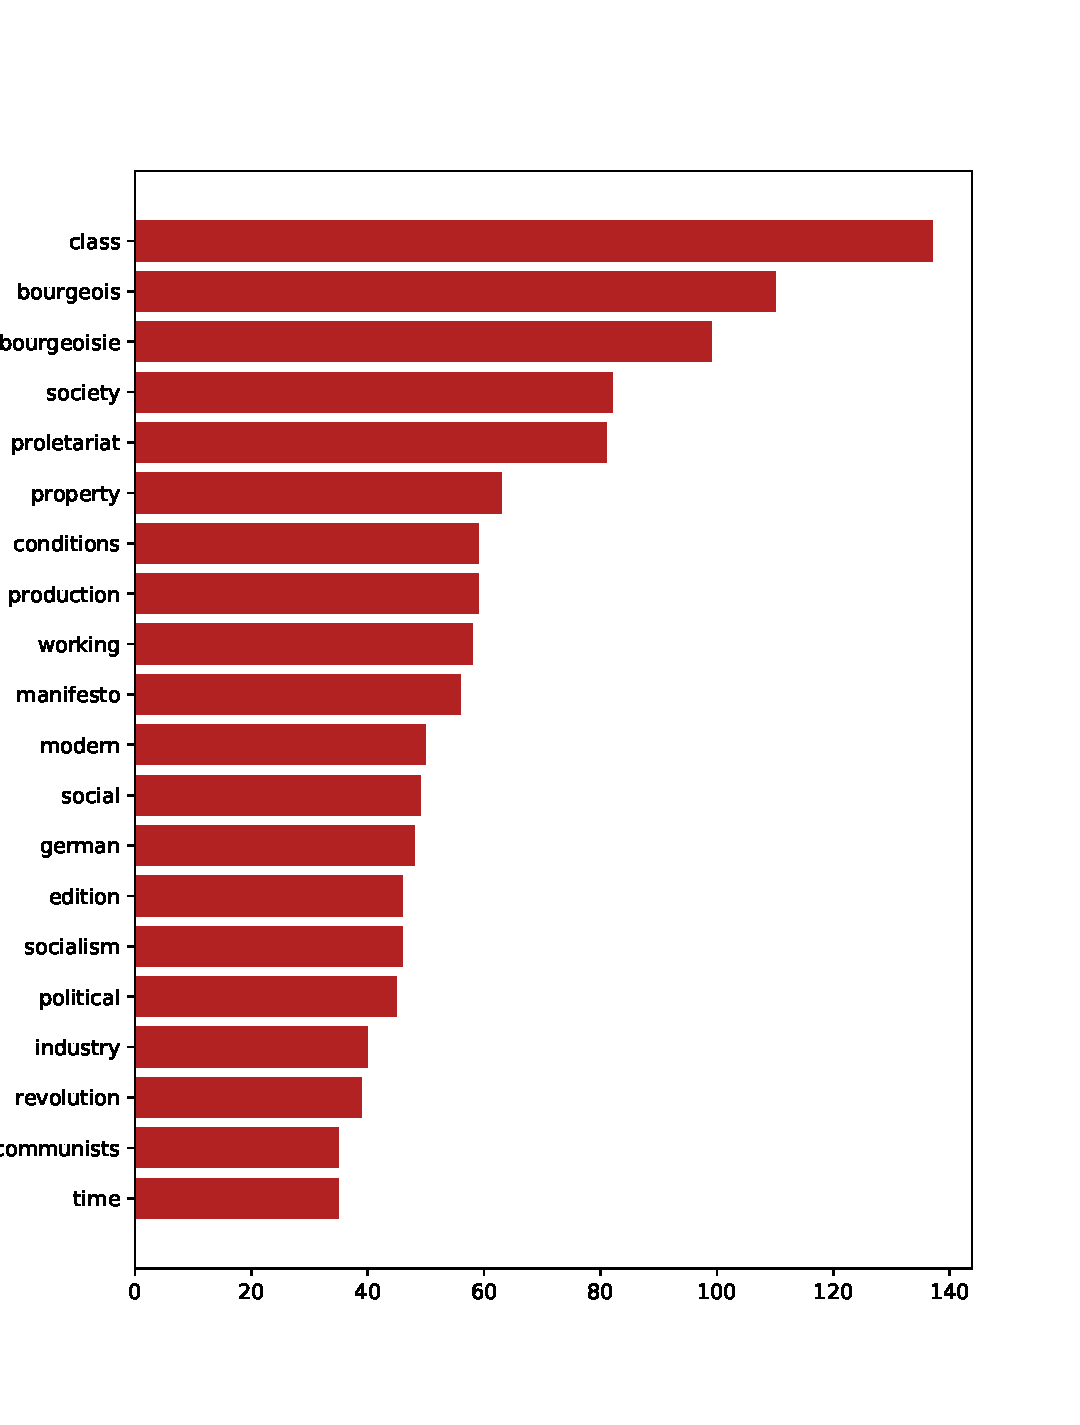
\includegraphics[width=0.9\linewidth]{figs/2004.epub-total}
    \caption{2004 edition's top-20 words according to the exact counter.}
    \label{fig:2004-20-exact}
\end{figure}


\begin{figure}[!ht]
    \centering
    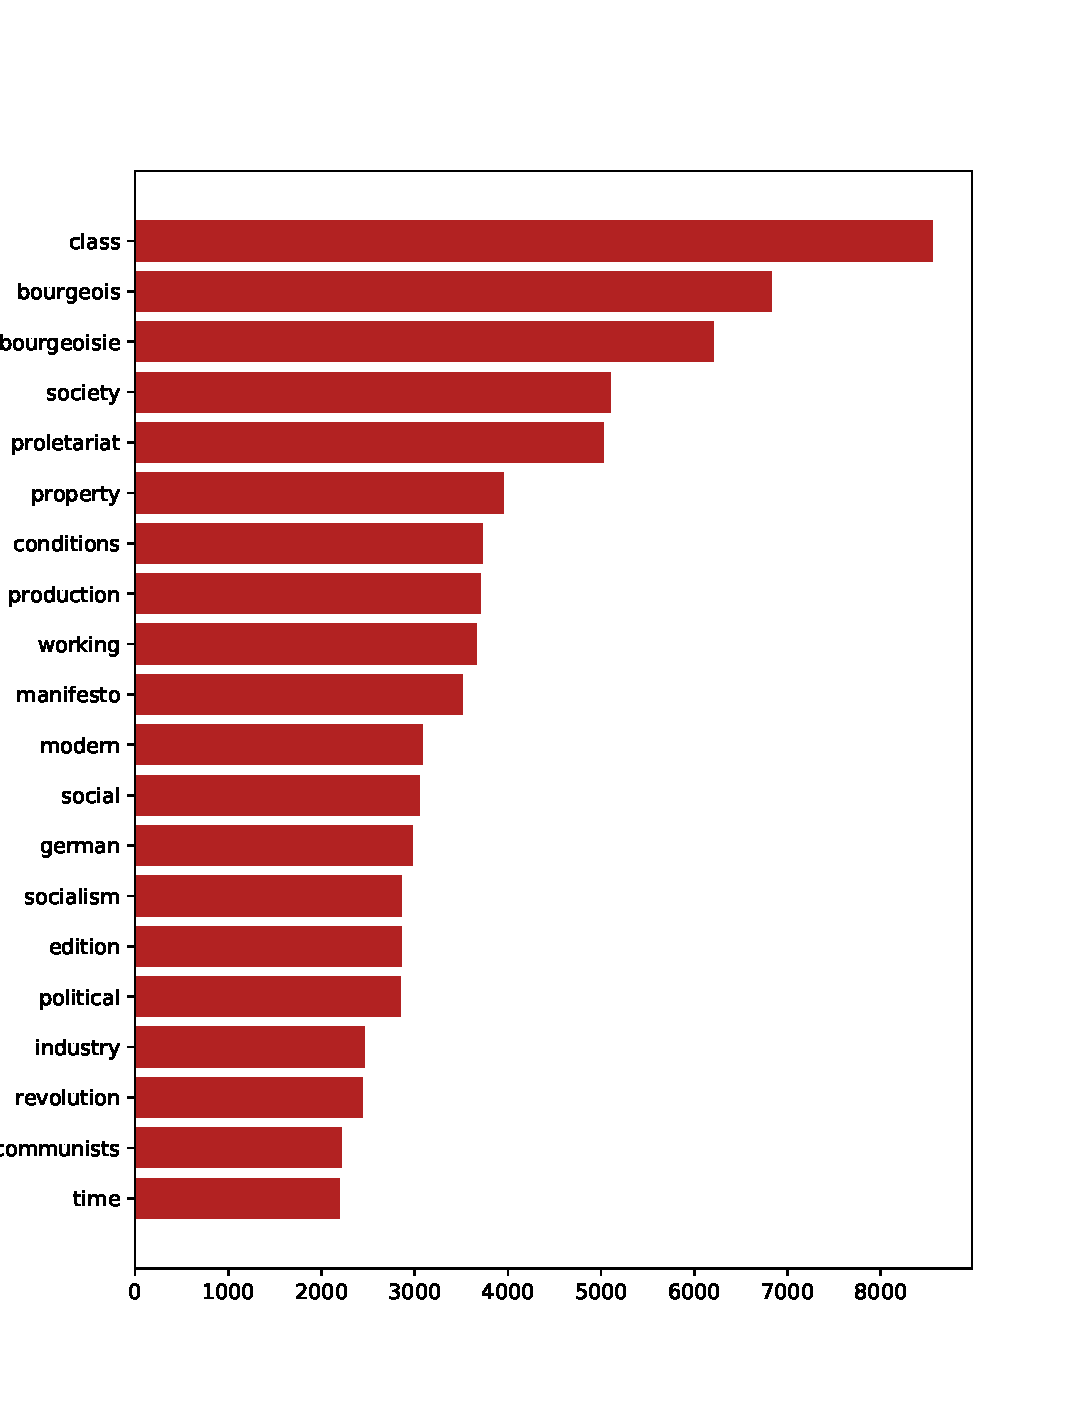
\includegraphics[width=0.9\linewidth]{figs/2004.epub-fixed-1000}
    \caption{2004 edition's top-20 words according to the average of one thousand fixed probability counters.}
    \label{fig:2004-20-fixed}
\end{figure}


\begin{figure}[!ht]
    \centering
    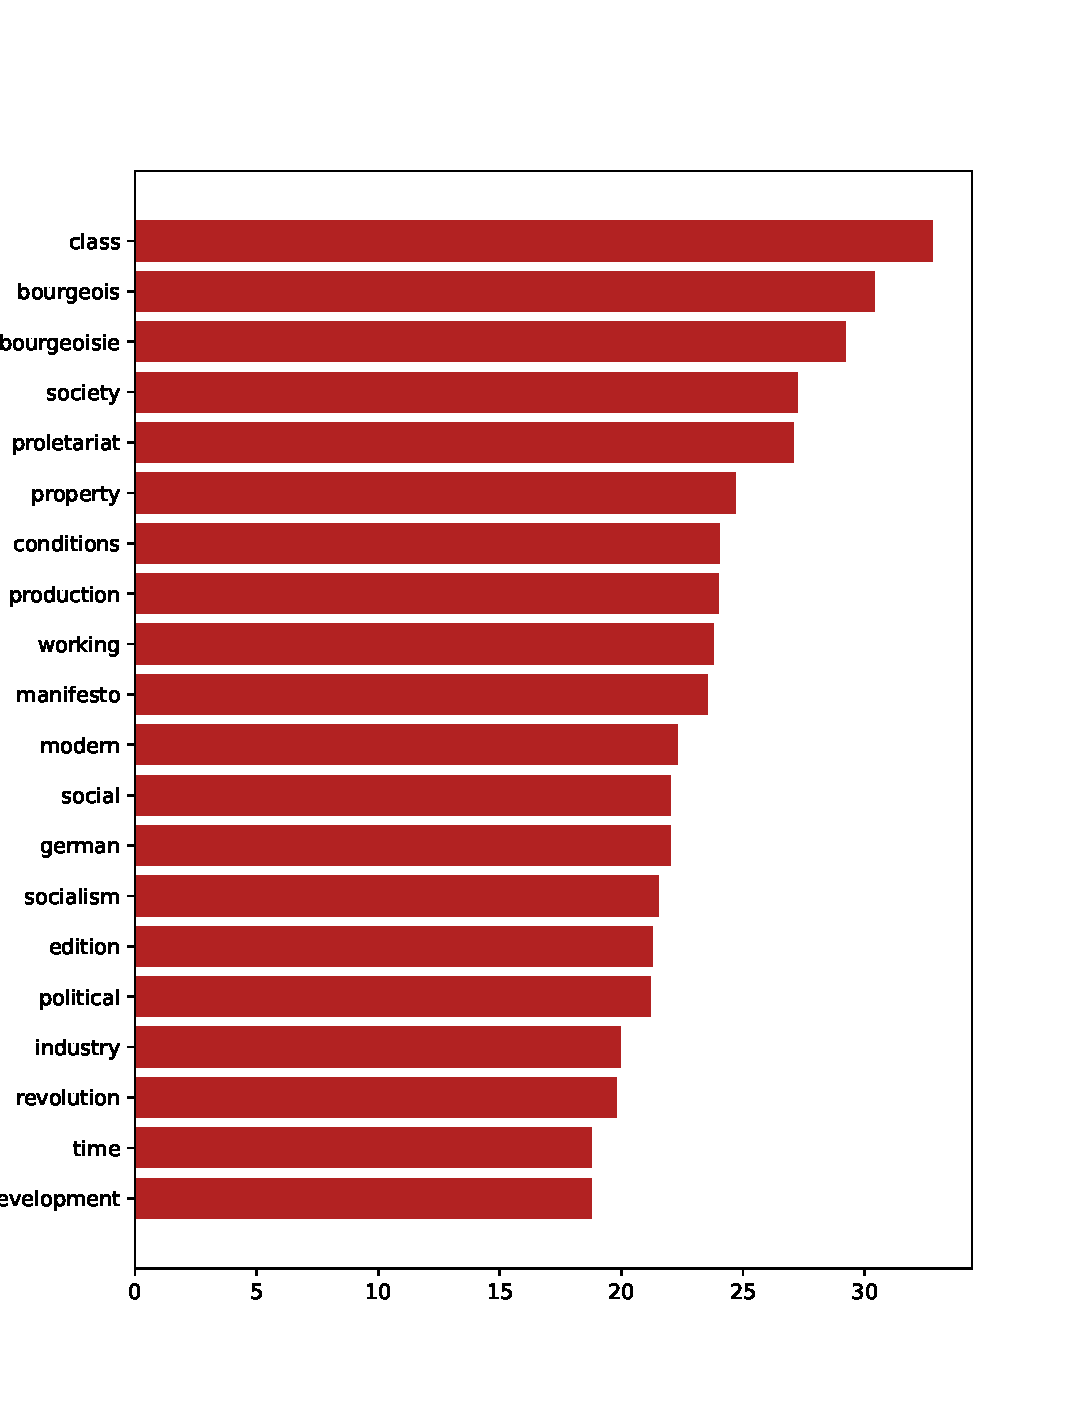
\includegraphics[width=0.9\linewidth]{figs/2004.epub-csuros-1000}
    \caption{2004 edition's top-20 words according to the average of one thousand Csűrös' counters.}
    \label{fig:2004-20-csuros}
\end{figure}


\autoref{tab:2004} presents the statistics of the top-3 words for the 2004 edition.
In this statistics we can observe that the difference between the expected and the mean counter values is slim.
It is also verifiable that the fixed probability counter present a larger standard deviation than the Csűrös's counter.
The mean relative error is smaller in the Csűrös' counter, while the mean accuracy ratio stands closer to the number one on the fixed probability counter.


\begin{table}[!ht]
    \centering
    \caption{Statistics of the top-3 words for the 2004 edition, according to the fixed probability counter (Fixed) and the Csűrös' Counter (Csűrös).}
    \label{tab:2004}
    \resizebox{\columnwidth}{!}{%
    \begin{tabular}{l|cc|cc|cc|}
    Word                   & \multicolumn{2}{c|}{Class}          & \multicolumn{2}{c|}{Bourgeois}      & \multicolumn{2}{c|}{Bourgeoisie}    \\ \hline
    Counter Type           & \multicolumn{1}{c|}{Fixed} & Csűrös & \multicolumn{1}{c|}{Fixed} & Csűrös & \multicolumn{1}{c|}{Fixed} & Csűrös \\ \hline
    Real Value             & \multicolumn{2}{c|}{137}            & \multicolumn{2}{c|}{110}            & \multicolumn{2}{c|}{99}             \\ \hline
    Expected Counter Value & \multicolumn{1}{c|}{34.25} & 33.06  & \multicolumn{1}{c|}{27.5}  & 30.75  & \multicolumn{1}{c|}{24.75} & 29.38  \\ \hline
    Mean Counter Value     & \multicolumn{1}{c|}{34.19} & 32.78  & \multicolumn{1}{c|}{27.68} & 30.41  & \multicolumn{1}{c|}{24.72} & 29.2   \\ \hline
    Standard Deviation     & \multicolumn{1}{c|}{4.96}  & 2.24   & \multicolumn{1}{c|}{4.52}  & 2.26   & \multicolumn{1}{c|}{4.25}  & 2.44   \\ \hline
    Maximum Absolute Error & \multicolumn{1}{c|}{18.75} & 9.06   & \multicolumn{1}{c|}{15.5}  & 6.75   & \multicolumn{1}{c|}{12.25} & 8.62   \\ \hline
    Mean Absolute Error    & \multicolumn{1}{c|}{3.95}  & 1.72   & \multicolumn{1}{c|}{3.675} & 1.88   & \multicolumn{1}{c|}{3.41}  & 2.03   \\ \hline
    Mean Relative Error    & \multicolumn{1}{c|}{0.115} & 0.051  & \multicolumn{1}{c|}{0.134} & 0.061  & \multicolumn{1}{c|}{0.138} & 0.069  \\ \hline
    Mean Accuracy Ratio    & \multicolumn{1}{c|}{0.998} & 0.991  & \multicolumn{1}{c|}{1.006} & 0.989  & \multicolumn{1}{c|}{0.999} & 0.994  \\ \hline
    Smallest Counter Value & \multicolumn{1}{c|}{19}    & 24     & \multicolumn{1}{c|}{15}    & 24     & \multicolumn{1}{c|}{14}    & 24     \\ \hline
    Largest Counter Value  & \multicolumn{1}{c|}{53}    & 40     & \multicolumn{1}{c|}{43}    & 37     & \multicolumn{1}{c|}{37}    & 38    
    \end{tabular}%
    }
    \end{table}
  
    
Additional data retrieved during the experience by using the \verb|sys.getsizeof()| function states that the exact counter takes 147568 bytes of memory, while the approximate counters only take on average 40 bytes.

\newpage
\subsection{2005 edition}

For the 2005 edition, the top-20 words calculated by the exact counter, an average of one thousand fixed probability counters, and an average of one thousand Csűrös' probability counters are shown in \autoref{fig:2005-20-exact}, \autoref{fig:2005-20-fixed}, and \autoref{fig:2005-20-csuros}, respectively.
From these graphs we can observe that the top-9 words are the same in every case. 
The first discrepancy seen is on the sixth position of \autoref{fig:2005-20-fixed} and \autoref{fig:2005-20-csuros}, where \emph{production} overtakes \emph{conditions}.
Both approximate counters present only four different relative positions in the graphs.
Every graph shares the same top-20 words.


\begin{figure}[!ht]
    \centering
    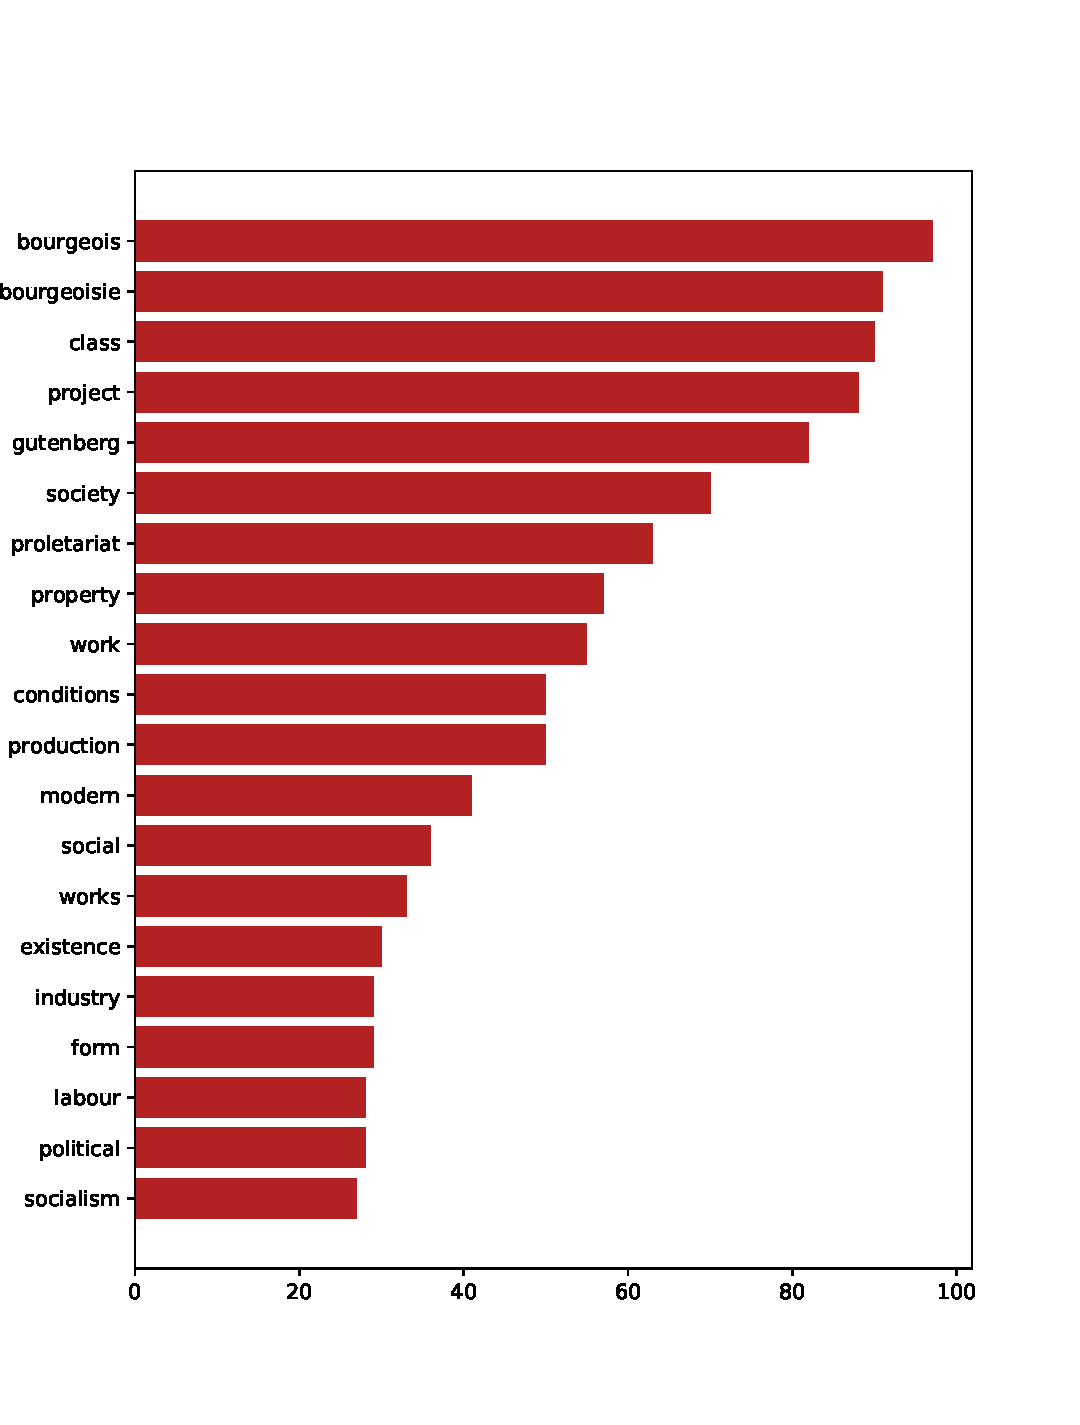
\includegraphics[width=0.9\linewidth]{figs/2005.epub-total}
    \caption{2005 edition's top-20 words according to the exact counter.}
    \label{fig:2005-20-exact}
\end{figure}


\begin{figure}[!ht]
    \centering
    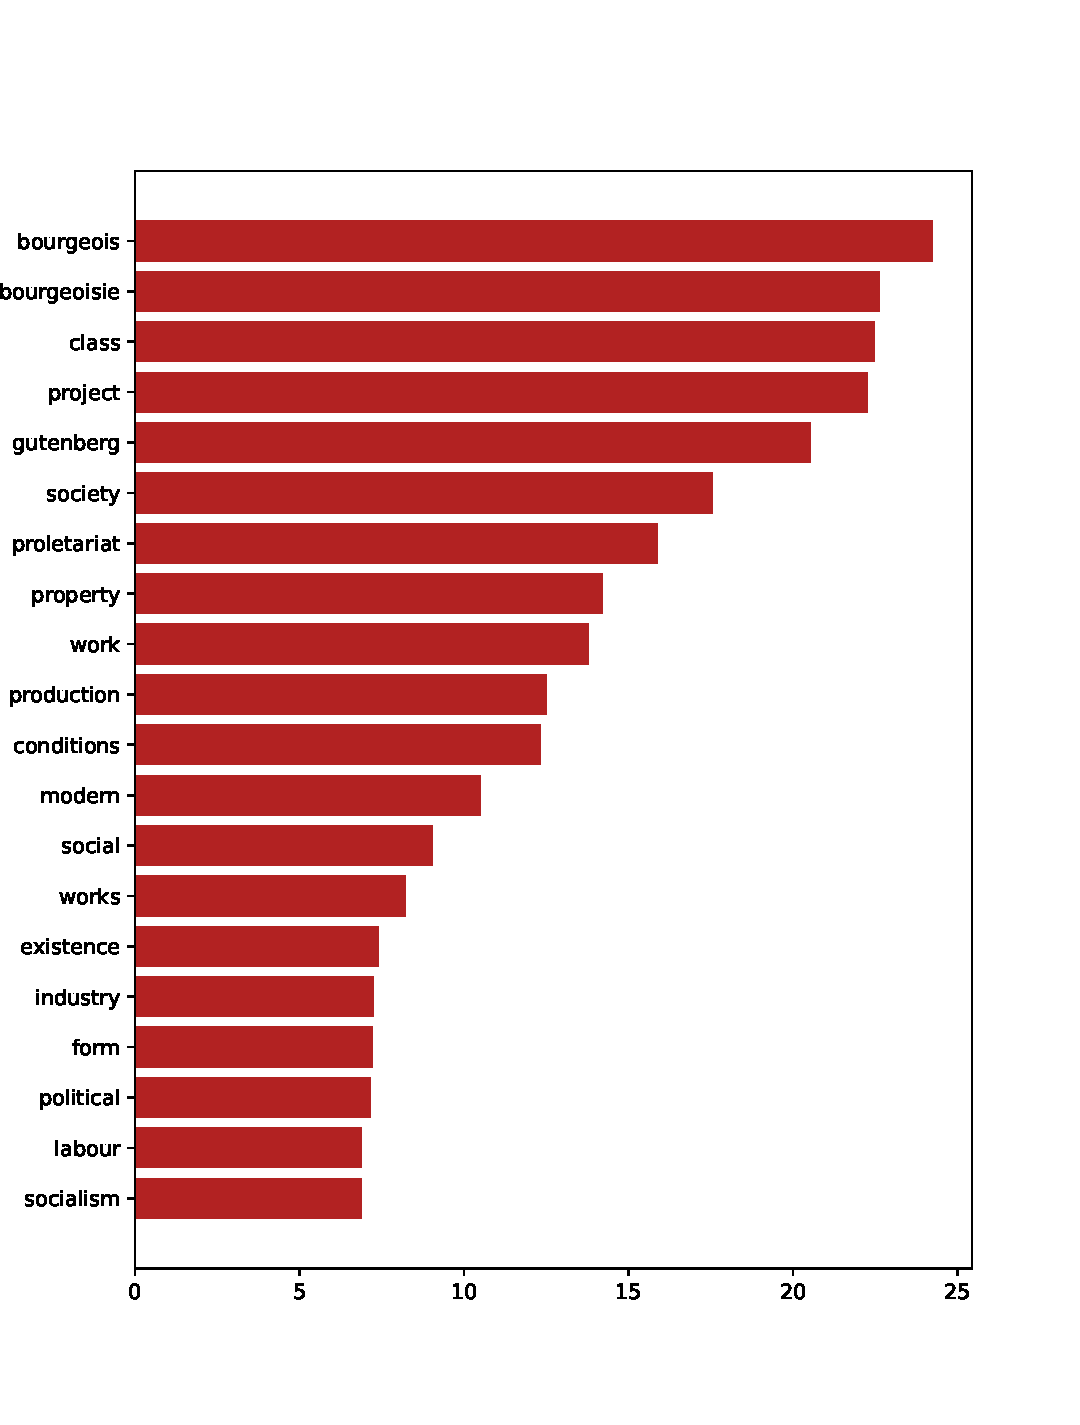
\includegraphics[width=0.9\linewidth]{figs/2005.epub-fixed-1000}
    \caption{2005 edition's top-20 words according to the average of one thousand fixed probability counters.}
    \label{fig:2005-20-fixed}
\end{figure}


\begin{figure}[!ht]
    \centering
    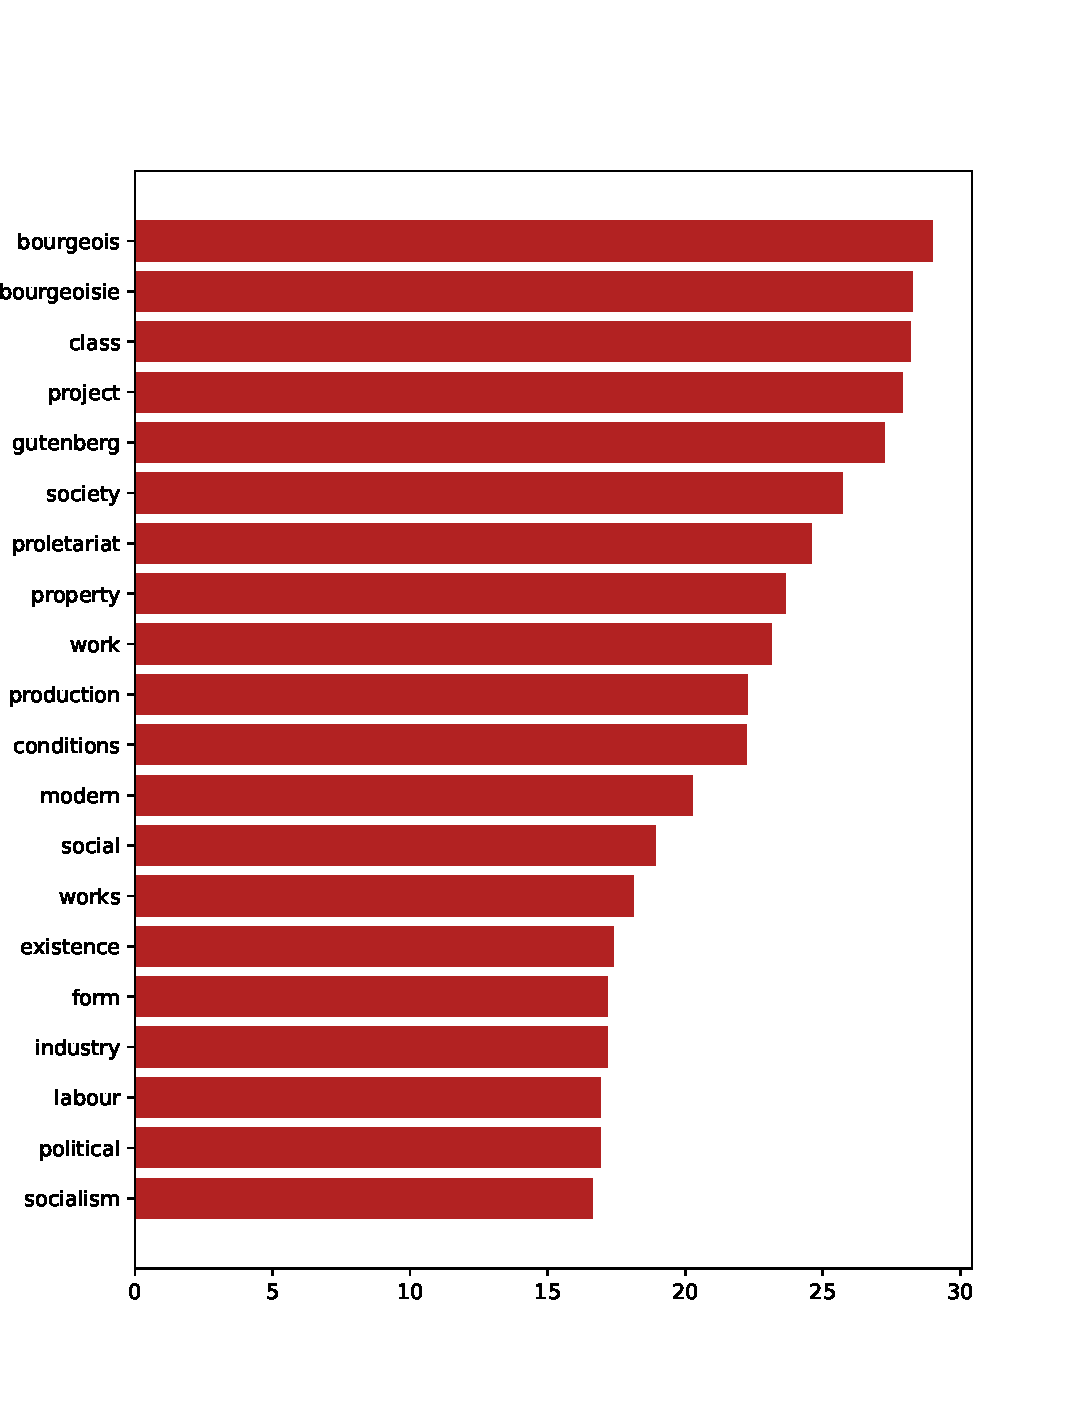
\includegraphics[width=0.9\linewidth]{figs/2005.epub-csuros-1000}
    \caption{2005 edition's top-20 words according to the average of one thousand Csűrös' counters.}
    \label{fig:2005-20-csuros}
\end{figure}


\autoref{tab:2005} presents the statistics of the top-3 words for the 2010 edition.
In this statistics we can observe that the difference between the expected and the mean counter values is slim.
Similarly to \autoref{tab:2004}, the fixed probability counter present a larger standard deviation than the Csűrös's counter and the mean relative error is smaller in the Csűrös' counter.
The mean accuracy ratio is similar between counters.


\begin{table}[!ht]
    \centering
    \caption{Statistics of the top-3 words for the 2005 edition, according to the fixed probability counter and the Csűrös' Counter.}
    \label{tab:2005}
    \resizebox{\columnwidth}{!}{%
    \begin{tabular}{l|cc|cc|cc|}
    Word                   & \multicolumn{2}{c|}{Bourgeois}       & \multicolumn{2}{c|}{Bourgeoisie}     & \multicolumn{2}{c|}{Class}          \\ \hline
    Counter Type           & \multicolumn{1}{c|}{Fixed}  & Csűrös & \multicolumn{1}{c|}{Fixed}  & Csűrös & \multicolumn{1}{c|}{Fixed} & Csűrös \\ \hline
    Real Value             & \multicolumn{2}{c|}{97}              & \multicolumn{2}{c|}{91}              & \multicolumn{2}{c|}{90}             \\ \hline
    Expected Counter Value & \multicolumn{1}{c|}{24.25}  & 29.12  & \multicolumn{1}{c|}{22.75}  & 28.38  & \multicolumn{1}{c|}{22.50} & 28.25  \\ \hline
    Mean Counter Value     & \multicolumn{1}{c|}{24.23}  & 28.98  & \multicolumn{1}{c|}{22.621} & 28.281 & \multicolumn{1}{c|}{22.49} & 28.2   \\ \hline
    Standard Deviation     & \multicolumn{1}{c|}{4.34}   & 2.36   & \multicolumn{1}{c|}{3.93}   & 2.27   & \multicolumn{1}{c|}{4.14}  & 2.23   \\ \hline
    Maximum Absolute Error & \multicolumn{1}{c|}{13.75}  & 6.88   & \multicolumn{1}{c|}{13.25}  & 6.62   & \multicolumn{1}{c|}{15.50} & 6.25   \\ \hline
    Mean Absolute Error    & \multicolumn{1}{c|}{3.466}  & 1.96   & \multicolumn{1}{c|}{3.14}   & 1.87   & \multicolumn{1}{c|}{3.31}  & 1.81   \\ \hline
    Mean Relative Error    & \multicolumn{1}{c|}{0.1429} & 0.067  & \multicolumn{1}{c|}{0.138}  & 0.066  & \multicolumn{1}{c|}{0.147} & 0.641  \\ \hline
    Mean Accuracy Ratio    & \multicolumn{1}{c|}{0.999}  & 0.995  & \multicolumn{1}{c|}{0.994}  & 0.997  & \multicolumn{1}{c|}{1.000} & 0.998  \\ \hline
    Smallest Counter Value & \multicolumn{1}{c|}{12}     & 23     & \multicolumn{1}{c|}{11}     & 23     & \multicolumn{1}{c|}{11}    & 22     \\ \hline
    Largest Counter Value  & \multicolumn{1}{c|}{38}     & 36     & \multicolumn{1}{c|}{36}     & 35     & \multicolumn{1}{c|}{38}    & 34    
    \end{tabular}%
    }
\end{table}


Similarly to the previous edition, additional data retrieved during the experience by using the \verb|sys.getsizeof()| function states that the exact counter takes 147568 bytes of memory, while the approximate counters only take on average 40 bytes.

\newpage
\subsection{2010 edition}

For the 2010 edition, the top-20 words calculated by the exact counter, an average of one thousand fixed probability counters, and an average of one thousand Csűrös' probability counters are shown in \autoref{fig:2010-20-exact}, \autoref{fig:2010-20-fixed}, and \autoref{fig:2010-20-csuros}, respectively.
From these graphs we can verify that they all share the same words in the same relative position.

\begin{figure}[!ht]
    \centering
    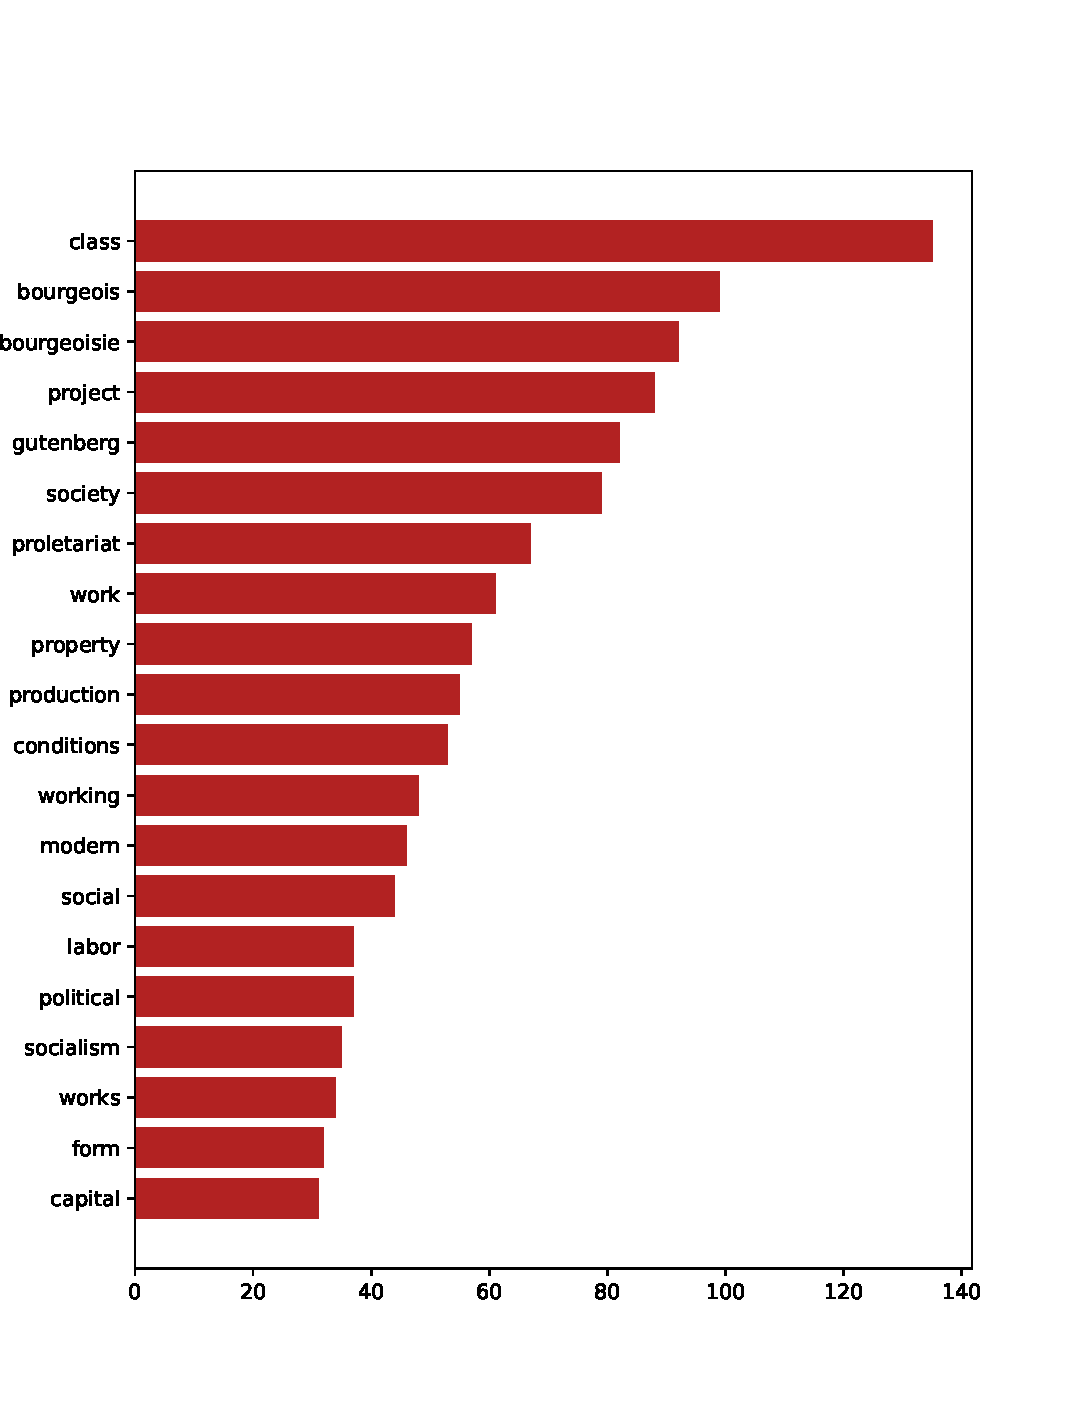
\includegraphics[width=0.9\linewidth]{figs/2010.epub-total}
    \caption{2010 edition's top-20 words according to the exact counter.}
    \label{fig:2010-20-exact}
\end{figure}


\begin{figure}[!ht]
    \centering
    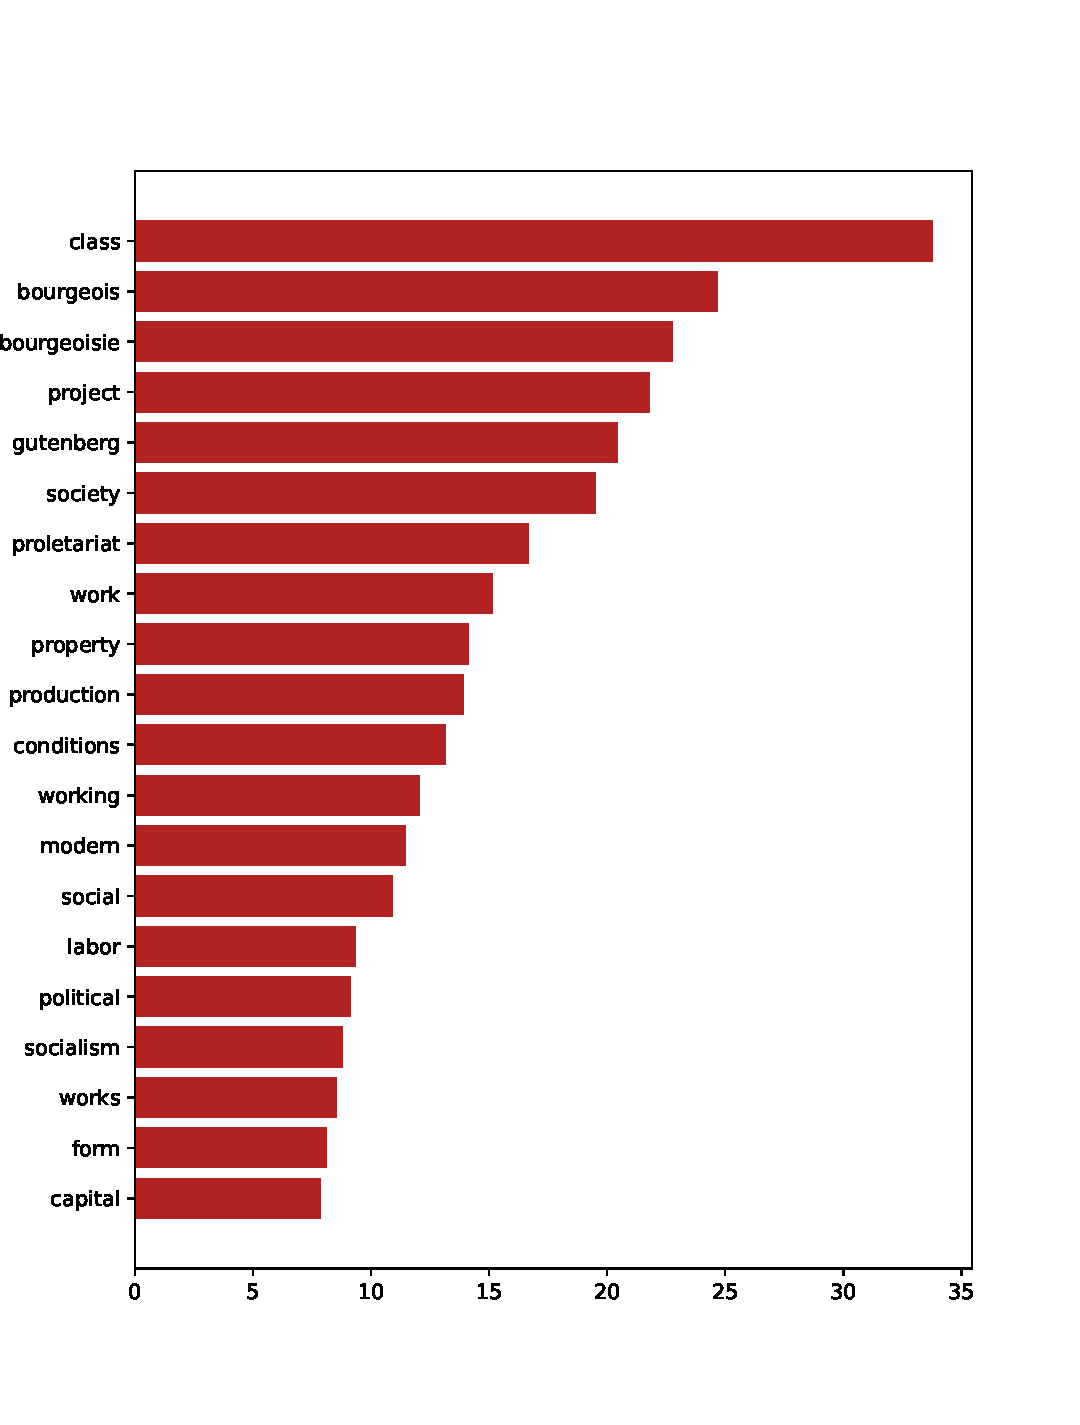
\includegraphics[width=0.9\linewidth]{figs/2010.epub-fixed-1000}
    \caption{2010 edition's top-20 words according to the average of one thousand fixed probability counters.}
    \label{fig:2010-20-fixed}
\end{figure}


\begin{figure}[!ht]
    \centering
    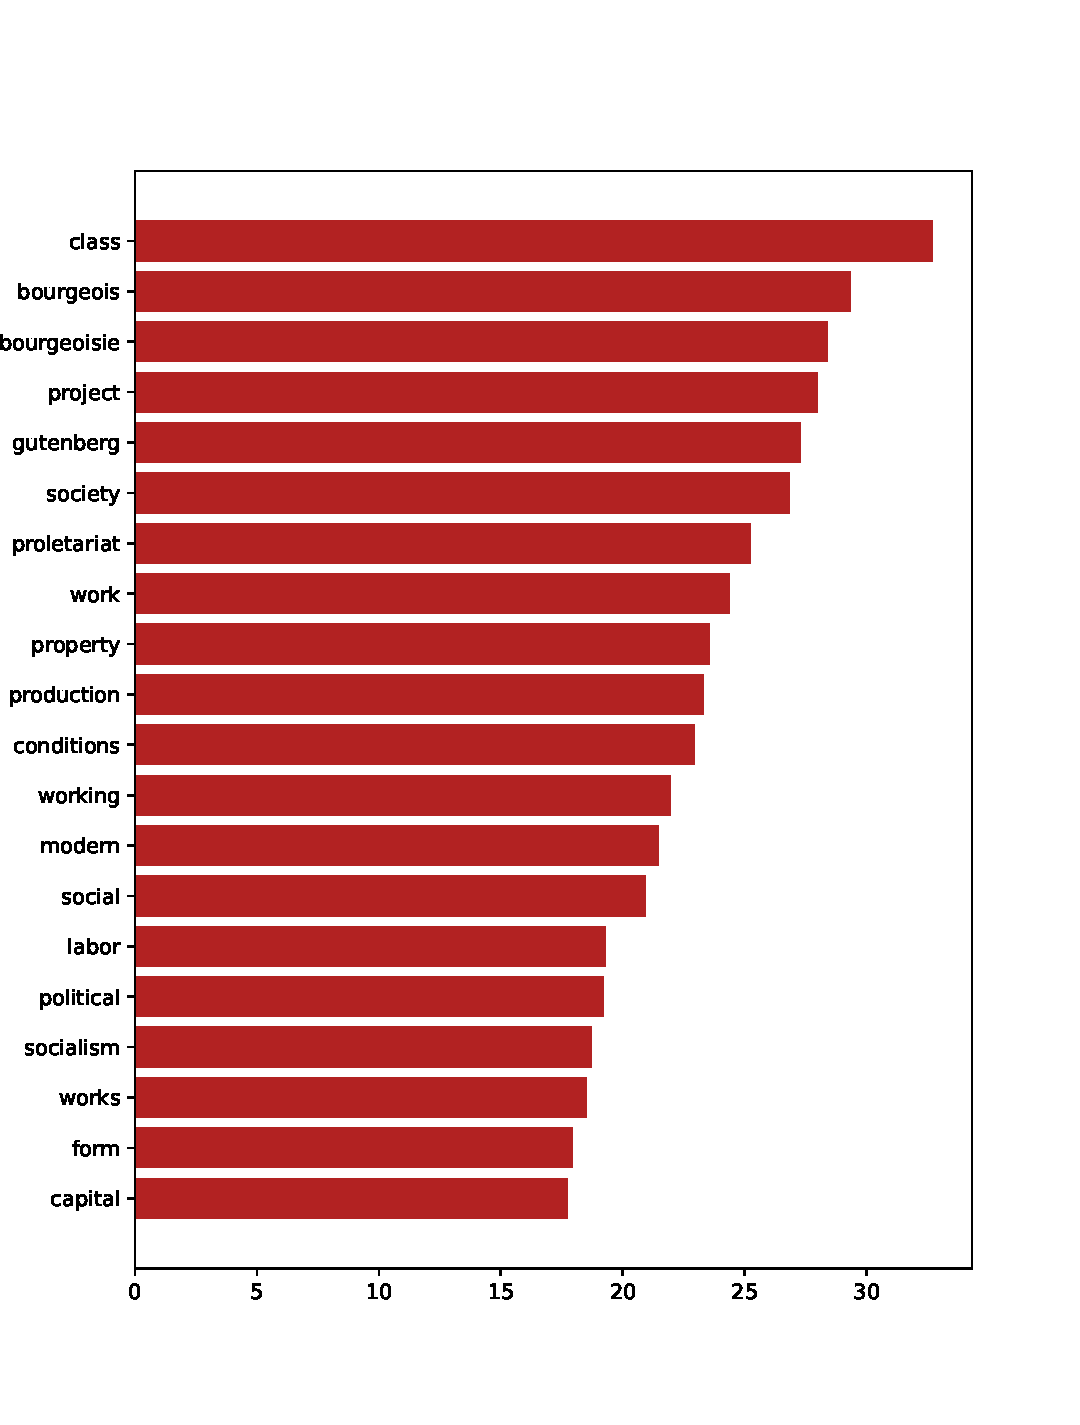
\includegraphics[width=0.9\linewidth]{figs/2010.epub-csuros-1000}
    \caption{2010 edition's top-20 words according to the average of one thousand Csűrös' counters.}
    \label{fig:2010-20-csuros}
\end{figure}


\autoref{tab:2010} presents the statistics of the top-3 words for the 2010 edition.
In this statistics we can observe that the difference between the expected and the mean counter values is slim, as seen in previous counters.
The observations taken for \autoref{tab:2005} can be taken here as well, from the larger standard deviation on the fixed probability counter to the smaller mean relative error in the Csűrös' counter.
\begin{table}[!ht]
\centering
\caption{Statistics of the top-3 words for the 2010 edition, according to the fixed probability counter and the Csűrös' Counter.}
\label{tab:2010}
\resizebox{\columnwidth}{!}{%
\begin{tabular}{l|cc|cc|cc|}
Word                   & \multicolumn{2}{c|}{Class}          & \multicolumn{2}{c|}{Bourgeois}      & \multicolumn{2}{c|}{Bourgeoisie}    \\ \hline
Counter Type           & \multicolumn{1}{c|}{Fixed} & Csűrös & \multicolumn{1}{c|}{Fixed} & Csűrös & \multicolumn{1}{c|}{Fixed} & Csűrös \\ \hline
Real Value             & \multicolumn{2}{c|}{135}            & \multicolumn{2}{c|}{99}             & \multicolumn{2}{c|}{92}             \\ \hline
Expected Counter Value & \multicolumn{1}{c|}{33.75} & 32.94  & \multicolumn{1}{c|}{24.75} & 29.38  & \multicolumn{1}{c|}{23.00} & 28.50  \\ \hline
Mean Counter Value     & \multicolumn{1}{c|}{33.77} & 32.69  & \multicolumn{1}{c|}{24.67} & 29.33  & \multicolumn{1}{c|}{22.79} & 28.38  \\ \hline
Standard Deviation     & \multicolumn{1}{c|}{4.97}  & 2.28   & \multicolumn{1}{c|}{4.37}  & 2.32   & \multicolumn{1}{c|}{4.14}  & 2.32   \\ \hline
Maximum Absolute Error & \multicolumn{1}{c|}{17.25} & 9.06   & \multicolumn{1}{c|}{15.25} & 7.62   & \multicolumn{1}{c|}{13.00} & 7.50   \\ \hline
Mean Absolute Error    & \multicolumn{1}{c|}{3.95}  & 1.70   & \multicolumn{1}{c|}{3.45}  & 1.91   & \multicolumn{1}{c|}{3.31}  & 1.90   \\ \hline
Mean Relative Error    & \multicolumn{1}{c|}{0.117} & 0.052  & \multicolumn{1}{c|}{0.140} & 0.065  & \multicolumn{1}{c|}{0.144} & 0.067  \\ \hline
Mean Accuracy Ratio    & \multicolumn{1}{c|}{1.000} & 0.992  & \multicolumn{1}{c|}{0.997} & 0.999  & \multicolumn{1}{c|}{0.991} & 0.996  \\ \hline
Smallest Counter Value & \multicolumn{1}{c|}{18}    & 24     & \multicolumn{1}{c|}{12}    & 22     & \multicolumn{1}{c|}{11}    & 21     \\ \hline
Largest Counter Value  & \multicolumn{1}{c|}{51}    & 42     & \multicolumn{1}{c|}{40}    & 37     & \multicolumn{1}{c|}{36}    & 36    
\end{tabular}%
}
\end{table}

Similarly to the previous subsections, additional data retrieved during the experience by using the \verb|sys.getsizeof()| function states that the exact counter takes 147568 bytes of memory, while the approximate counters only take on average 40 bytes.

\newpage